% !TeX program = pdflatex
% Versioni 4 (Faza 2) - IEEEtran Conference.
% Për Overleaf: Menu -> Compiler -> pdfLaTeX.
% Burimet kryesore të kontekstit: Strategjia e Kosovës për Qeverisje Elektronike
% 2023-2027, Agjenda Digjitale e Kosovës 2030 dhe studimi KIPRED/DCAF (2022).
% Ndryshimet ndaj versionit 3: punim i orientuar nga objektivat (pa pyetje
% kërkimore), metodat e hulumtimit, teknologjitë dhe veglat, përshkrimi i
% problemit, vlerësimi paraprak i modelit, SWOT/TOWS qendror--lokal,
% rezultatet e pritura dhe punime të reja shkencore (2019--2026).
\documentclass[conference]{IEEEtran}
\usepackage[T1]{fontenc}
\usepackage[utf8]{inputenc}
\usepackage[albanian]{babel}
\usepackage{newtxtext}
\usepackage{cite}
\usepackage{graphicx}
\usepackage{booktabs}
\usepackage{array}
\usepackage{tabularx}
\usepackage{url}
\usepackage{tikz}
\usetikzlibrary{arrows.meta,positioning}
\usepackage{hyperref}
\hypersetup{hidelinks}
% babel i rivendos emërtimet në \begin{document}, prandaj \addto
\addto\captionsalbanian{%
  \renewcommand{\abstractname}{Abstrakti}%
  \renewcommand{\refname}{Referencat}%
  \renewcommand{\tablename}{Tabela}%
  \renewcommand{\figurename}{Figura}%
}
\renewcommand{\IEEEkeywordsname}{Fjalët kyçe}
\newcolumntype{L}[1]{>{\raggedright\arraybackslash}p{#1}}
\newcolumntype{Y}{>{\raggedright\arraybackslash}X}
% Ndarja e autorëve në dy rreshta sipas renditjes në dokumentin origjinal.
\makeatletter
\newcommand{\linebreakand}{%
  \end{@IEEEauthorhalign}%
  \hfill\mbox{}\par
  \vspace{0.9em}%
  \mbox{}\hfill\begin{@IEEEauthorhalign}%
}
\makeatother
\begin{document}
% ---------------------------------------------------------------------
% 1. TITULLI I PUNIMIT
% ---------------------------------------------------------------------
\title{Modelet, korniza e mundësive dhe sfidat e e-Qeverisjes\\
në Kosovë: Vlerësim i integruar dhe propozim\\
për përmirësimin e koordinimit ndërinstitucional}
% Blloqet individuale të autorëve në formatin IEEE Conference: 3 + 2.
\author{
\IEEEauthorblockN{Shefket Bylygbashi}
\IEEEauthorblockA{\textit{Inxhinieri Kompjuterike}\\
\textit{dhe Softuerike}\\
\textit{Fakulteti i Inxhinierisë Elektrike}\\
\textit{dhe Kompjuterike}\\
Prishtinë, Kosovë\\
{\textit{shefket.bylygbashi@student.uni-pr.edu}}}\\
\and
\IEEEauthorblockN{Rinor Ukshini}
\IEEEauthorblockA{\textit{Inxhinieri Kompjuterike}\\
\textit{dhe Softuerike}\\
\textit{Fakulteti i Inxhinierisë Elektrike}\\
\textit{dhe Kompjuterike}\\
Prishtinë, Kosovë\\
{\textit{rinor.ukshini1@student.uni-pr.edu}}}\\
\and
\IEEEauthorblockN{Arton Gërguri}
\IEEEauthorblockA{\textit{Inxhinieri Kompjuterike}\\
\textit{dhe Softuerike}\\
\textit{Fakulteti i Inxhinierisë Elektrike}\\
\textit{dhe Kompjuterike}\\
Prishtinë, Kosovë\\
{\textit{arton.gerguri@student.uni-pr.edu}}}\\
\linebreakand
\IEEEauthorblockN{Rina Bunjaku}
\IEEEauthorblockA{\textit{Inxhinieri Kompjuterike}\\
\textit{dhe Softuerike}\\
\textit{Fakulteti i Inxhinierisë Elektrike}\\
\textit{dhe Kompjuterike}\\
Prishtinë, Kosovë\\
{\textit{rina.bunjaku@student.uni-pr.edu}}}\\
\and
\IEEEauthorblockN{Besarta Berisha}
\IEEEauthorblockA{\textit{Inxhinieri Kompjuterike}\\
\textit{dhe Softuerike}\\
\textit{Fakulteti i Inxhinierisë Elektrike}\\
\textit{dhe Kompjuterike}\\
Prishtinë, Kosovë\\
{\textit{besarta.berisha1@student.uni-pr.edu}}}\\
}
\maketitle
% Abstrakti do të plotësohet pasi të përfundojë punimi.
% \begin{abstract}
% \end{abstract}
% ---------------------------------------------------------------------
% 2. FJALËT KYÇE
% ---------------------------------------------------------------------
\begin{IEEEkeywords}
e-Qeverisja, maturia digjitale, ndërveprueshmëria, analiza SWOT--TOWS,
qeverisja shumënivelëshe, koordinimi ndërinstitucional
\end{IEEEkeywords}
% ---------------------------------------------------------------------
% 3. HYRJE
% ---------------------------------------------------------------------
\section{Hyrje}
\label{sec:hyrje}
Transformimi digjital i sektorit publik nuk është më një projekt
teknologjik, por një reformë institucionale që prek mënyrën se si shteti
organizon kompetencat, proceset dhe marrëdhënien me qytetarin
\cite{mergel2019}. Kur një procedurë kërkon të dhëna nga dy institucione,
cilësia e shërbimit nuk varet vetëm nga portali, por edhe nga marrëveshja
ndërmjet tyre: dikush duhet ta mbajë të saktë regjistrin, të përcaktojë kush
ka të drejtë ta përdorë dhe t'i përgjigjet qytetarit kur ndodh një gabim.
Literatura për evolucionin e qeverisjes digjitale e përshkruan këtë
zhvendosje si kalim nga digjitalizimi i proceseve të brendshme te
transformimi, angazhimi dhe, në fund, kontekstualizimi i politikave sipas
nevojave të vendit \cite{janowski2015}. Për vendet e vogla, peshën kryesore
në suksesin e projekteve e kanë kushtet organizative, politike e ligjore,
jo vetëm gatishmëria teknike \cite{glyptis2020}.

Kosova përbën një rast studimi veçanërisht të pasur për këtë problematikë.
Vendi ka ndërtuar një trajektore të qëndrueshme strategjike: nga Strategjia
e parë e Qeverisjes Elektronike 2009--2015 dhe Agjenda Digjitale 2013--2020,
te anëtarësimi në Agjendën Digjitale të BE-së për Ballkanin Perëndimor
(2018) dhe Strategjia e Reformës së Administratës Publike (RAP) 2022--2027
\cite{strategjia2023}. Kjo trajektore kulmon me Agjendën Digjitale të
Kosovës 2030 (AD~2030), një agjendë horizontale ndërsektoriale me pesë
objektiva strategjikë dhe buxhet indikativ prej 152 milionë eurosh
\cite{agjenda2030}, si dhe me Strategjinë e Kosovës për Qeverisje
Elektronike 2023--2027, të hartuar me mbështetjen e Akademisë Estoneze të
e-Qeverisjes dhe të strukturuar në gjashtë objektiva: koordinimi e
menaxhimi, kompetencat digjitale, ndërveprueshmëria, shërbimet digjitale,
siguria kibernetike dhe inovacioni \cite{strategjia2023}. Në rrafshin
teknik, ekosistemi mbështetet në rrjetin e dedikuar qeveritar, në platformën
e ndërveprueshmërisë \textit{Government Gateway} (funksionale që nga viti
2017) dhe në portalin e-Kosova si dritare e vetme për shërbimet e të gjitha
niveleve të qeverisjes. Baza ligjore përfshin, ndër të tjera, Ligjin
Nr.~04/L-094 për shërbimet e shoqërisë së informacionit, Ligjin Nr.~08/L-022
për identifikimin elektronik dhe shërbimet e besuara, të përafruar me
eIDAS, dhe Ligjin Nr.~06/L-082 për mbrojtjen e të dhënave personale, të
përafruar me GDPR \cite{strategjia2023}. Procesi i integrimit evropian, i
formalizuar me Marrëveshjen e Stabilizim-Asociimit (2016) dhe me aplikimin
për anëtarësim në BE (2022) \cite{ec2024}, e shndërron përafrimin me
Kornizën Evropiane të Ndërveprueshmërisë (EIF) \cite{eif2017} nga një
zgjedhje politike në një detyrim strategjik.

Megjithatë, të dhënat e vetë dokumenteve strategjike zbulojnë një paradoks
ndërmjet lidhshmërisë dhe përdorimit (Tabela~\ref{tab:treguesit}). Ndonëse
pothuajse të gjitha ekonomitë familjare kanë qasje në internet, vetëm
5.3\% e përdoruesve të internetit kanë dorëzuar formularë online, ndërsa nga
mbi 700 shërbime që ofrojnë institucionet qendrore dhe lokale vetëm rreth
10\% ofrohen online \cite{strategjia2023,agjenda2030}. Sipas OECD-së, në vitin
2022 72\% e individëve nuk e kishin përdorur internetin për informata ose
shërbime të administratës publike \cite{oecd2024}. Në Indeksin e Maturitetit
GovTech (GTMI) të Bankës Botërore, Kosova ka kaluar nga grupi C në grupin B,
kryesisht falë ofrimit të shërbimeve, por mbetet më e dobët pikërisht te
mundësuesit institucionalë (GTEI) dhe angazhimi digjital i qytetarëve
\cite{strategjia2023}. Kufizimi kryesor, pra, nuk është infrastruktura, por
kapaciteti institucional për ta shndërruar atë në vlerë publike.

\begin{table}[!t]
\caption{Treguesit kryesorë të gjendjes dhe synimet e e-Qeverisjes në
Kosovë sipas dokumenteve strategjike}
\label{tab:treguesit}
\centering
\footnotesize
\renewcommand{\arraystretch}{1.2}
\begin{tabular}{L{0.56\columnwidth} L{0.34\columnwidth}}
\toprule
\textbf{Treguesi} & \textbf{Vlera / synimi} \\
\midrule
Ekonomi familjare me qasje në internet \cite{strategjia2023} &
99.8\% (2021--2022) \\
Përdorues të internetit që kanë dorëzuar formularë online
\cite{agjenda2030} & 5.3\% (vlerë bazë, 2020) \\
Shërbime (nga mbi 700, qendrore e lokale) të ofruara online
\cite{strategjia2023} & $\approx$10\% (2023) \\
Shërbime qendrore e lokale të digjitalizuara -- synim
\cite{strategjia2023} & 40\% (2025); 65\% (2027) \\
Sisteme informative të lidhura me \textit{Government Gateway} -- synim
\cite{strategjia2023} & 30\% (2025); 70\% (2027) \\
Indeksi i mundësuesve GovTech (GTEI) \cite{strategjia2023} &
0.456, niveli C; synim $\geq$0.70 (2027) \\
Specialistë të TI-së në sektorin publik \cite{strategjia2023} &
$\approx$450, ose 0.5\% e punësimit publik (norma ndërkombëtare 2--3\%) \\
Buxheti indikativ i AD~2030 \cite{agjenda2030} &
152 mln euro, prej tyre 35\% nga donatorët \\
\bottomrule
\end{tabular}
\end{table}

Ky hendek shfaqet në tri dimensione të ndërlidhura. \textit{Horizontalisht},
shumë shërbime ofrohen përmes portaleve individuale të agjencive, metadatat
nuk janë të harmonizuara, nuk ekziston një pasqyrë e sistemeve të TI-së në
sektorin publik dhe arkitektura e ndërmarrjes së ``qeverisë në tërësi''
mungon ose është e vjetruar \cite{strategjia2023}; vlerësimi i Agjendës
2013--2020 tregoi gjithashtu se ministritë i zbatuan detyrat e tyre në
mënyra shumë të ndryshme, pa mekanizma korrigjues \cite{agjenda2030}.
\textit{Vertikalisht}, 38 komunat kanë kompetenca vetanake dhe të deleguara
në ofrimin e shërbimeve sipas Ligjit Nr.~03/L-040 për vetëqeverisjen lokale
(p.sh., neni~18 e rendit regjistrimin civil ndër kompetencat e deleguara)
\cite{ligji03L040}, por kapacitete digjitale shumë të pabarabarta, ndërkohë
që në përshkrimin e strukturave të zbatimit të Strategjisë 2023--2027 niveli
lokal nuk ka përfaqësim të dedikuar \cite{strategjia2023}.
\textit{Institucionalisht}, arkitektura e koordinimit mbështetet në
Komisionin për Transformim Digjital të kryesuar nga Kryeministri, Njësinë e
Transformimit Digjital, komitetin teknik dhe Këshillin e RAP-it
\cite{strategjia2023}. Ndërkohë, kalimi i Agjencisë së Shoqërisë së
Informacionit (ASHI) në kuadër të Ministrisë së Digjitalizimit dhe
Administratës Publike përfaqëson një hap të ri drejt konsolidimit
institucional; AD~2030 parashikon, nga ana e saj, raportim vjetor nga Zyra e
Kryeministrit dhe Ministria e Ekonomisë \cite{agjenda2030}, ndërsa në fushën
e sigurisë kibernetike veprojnë akterë të tjerë, si KOS-CERT, i cili sipas
gjendjes së vitit 2022 funksiononte në kuadër të ARKEP-it \cite{kipred2022}.
Vetë regjistri i rreziqeve të Strategjisë pranon se rolet e palëve janë të
paqarta dhe se ka fusha të mbivendosura, ndërsa menaxhimi i mundësuesve
kryesorë teknikë (identiteti digjital, \textit{Government Gateway}, e-Kosova
dhe qendra e të dhënave) varet nga partnerët e jashtëm \cite{strategjia2023}.

Situata rëndohet nga një deficit i matjes. Meqë Kosova nuk është shtet
anëtar i OKB-së, ajo nuk përfshihet në Indeksin e Zhvillimit të
e-Qeverisjes (EGDI) \cite{undesa2024} dhe ende nuk është pjesë e indeksit
DESI të BE-së \cite{agjenda2030}; njëkohësisht, shumë tregues të Strategjisë
2023--2027 kanë vlerë bazë ``N/A'' ose ``për t'u matur'' dhe trajtohen si
projekt-sugjerime deri në hartimin e Pasaportës së Treguesve
\cite{strategjia2023}. Pasojë metodologjike e kësaj është se një synim
përqindjeje ka vlerë krahasuese vetëm kur ekziston një matje për të njëjtin
vit dhe me të njëjtin përkufizim. Studimet akademike për Kosovën janë
kryesisht juridike ose të përqendruara te pranimi i shërbimeve
\cite{dermaku2024,krasniqi2026} dhe rrallë e lidhin maturinë e shërbimeve me
kornizën ligjore e institucionale dhe me dinamikat qendër--komunë.
% ---------------------------------------------------------------------
% 4. QËLLIMI I PUNIMIT
% ---------------------------------------------------------------------
\section{Qëllimi i punimit}
\label{sec:qellimi}
Qëllimi i këtij punimi është të vlerësojë në mënyrë kritike modelin aktual
të e-Qeverisjes në Kosovë dhe të identifikojë kushtet ligjore,
institucionale dhe organizative që e mundësojnë ose e pengojnë kalimin nga
digjitalizimi i shërbimeve të veçanta drejt një sistemi të integruar, të
sigurt dhe të orientuar te përdoruesi, në nivel qendror dhe lokal.
E-Qeverisja konceptualizohet si sistem socio-teknik, rezultatet e të cilit
varen nga ndërveprimi i politikave, menaxhimit dhe teknologjisë
\cite{pardo2012}. Kuadri analitik ndërthur modelin e fazave të Layne dhe Lee
\cite{layne2001} dhe modelin evolutiv të Janowskit \cite{janowski2015}, të
rishqyrtuar në literaturën e fundit si konfigurime jo-lineare të maturisë
\cite{iannacci2025}, me katër shtresat e ndërveprueshmërisë të EIF-it
(ligjore, organizative, semantike dhe teknike) për hartëzimin e kornizës
normative dhe institucionale \cite{eif2017}.

Punimi është i orientuar nga objektivat: në vend që të testojë një hipotezë
apo t'i përgjigjet një pyetjeje të vetme kërkimore, ai synon të prodhojë
katër rezultate analitike të përcaktuara paraprakisht (Seksioni~\ref{sec:objektivat}),
secili me metodë, dëshmi dhe kriter vlerësimi të vetin
(Tabela~\ref{tab:objmet}). Synimi përfundimtar është t'u ofrohet
politikëbërësve një bazë analitike dhe një udhërrëfyes i zbatueshëm, në
përputhje me afatet e Strategjisë 2023--2027 dhe të AD~2030.
% ---------------------------------------------------------------------
% 5. OBJEKTIVAT E PUNIMIT
% ---------------------------------------------------------------------
\section{Objektivat e punimit}
\label{sec:objektivat}
\begin{enumerate}
\renewcommand{\labelenumi}{O\arabic{enumi}:}
\item të vlerësohet niveli i maturisë së modelit aktual të e-Qeverisjes në
dimensionin horizontal (ndërsektorial) dhe vertikal (qendër--komunë) dhe të
formulohen rekomandime;
\item të hartëzohen boshllëqet, mbivendosjet e mandateve dhe mospërputhjet e
kornizës ligjore e institucionale sipas shtresave të EIF-it dhe kërkesave
përkatëse të \textit{acquis}-së së BE-së;
\item të kryhet një analizë krahasuese SWOT për nivelin qendror dhe atë
lokal, e zgjeruar në matricë TOWS;
\item të propozohet një model qeverisjeje për koordinimin ndërinstitucional,
me role, instrumente dhe tregues të matshëm të performancës.
\end{enumerate}
% ---------------------------------------------------------------------
% 6. GJENDJA AKTUALE (STATE OF THE ART)
% ---------------------------------------------------------------------
\section{Gjendja aktuale e punëve të ngjashme (State of the Art)}
\label{sec:sota}
\subsection{Maturia dhe faktorët e zbatimit}
Literatura e hershme e konceptualizon e-Qeverisjen si proces me faza. Layne
dhe Lee \cite{layne2001} dallojnë katalogimin, transaksionin, integrimin
vertikal dhe integrimin horizontal, duke argumentuar se çdo fazë rrit
kompleksitetin teknologjik e organizativ, por edhe vlerën për qytetarin.
Lee e zhvendos fokusin nga teknologjia te
institucionet përmes një modeli evolutiv katërfazor (digjitalizim,
transformim, angazhim, kontekstualizim), ku faza më e avancuar kërkon
përshtatjen e politikave me nevojat specifike të vendit dhe të komunitetit.
Kalimi ndërmjet fazave nuk është linear: Glyptis et al. gjen se në
komuna e-Qeverisja mbetet kryesisht në fazat informative e transaksionale
dhe se madhësia e kapacitetet administrative ndikojnë ndjeshëm. Për vendet
e vogla, Glyptis et al. \cite{glyptis2020} e lidhin suksesin e projekteve me
gatishmërinë elektronike, kornizën politike e ligjore dhe faktorët
organizativë e socio-kulturorë.

\subsection{Ndërveprueshmëria dhe koordinimi}
Linja e dytë e trajton integrimin si problem qeverisjeje. Pardo, Nam dhe
Burke \cite{pardo2012} tregojnë empirikisht se ndërveprueshmëria është
rezultat i ndërveprimit të politikave, menaxhimit dhe teknologjisë, ku
qeverisja e përbashkët dhe besimi ndërinstitucional janë po aq të
rëndësishëm sa standardet teknike. Rasti i Estonisë, model referimi për
Strategjinë kosovare, tregon se suksesi lidhet më shumë me vendimet e hershme
arkitekturore, kulturën e inovacionit dhe bashkëpunimin publik--privat sesa
me vëllimin e investimeve \cite{kalvet2012}.

\subsection{Studimet për Kosovën dhe boshllëku kërkimor}
Dërmaku dhe Emini \cite{dermaku2024} analizojnë bazën juridike të
digjitalizimit të administratës dhe tregojnë se transformimi kërkon
përputhje ndërmjet teknologjisë dhe normave të procedurës administrative,
regjistrave publikë dhe mbrojtjes së të dhënave. Krasniqi, Elezi dhe Vuniqi
\cite{krasniqi2026} identifikojnë besimin institucional, aftësitë digjitale,
interoperabilitetin dhe sigurinë kibernetike si sfidat kryesore të
platformës e-Kosova. Në dimensionin e sigurisë, Peci dhe Ukshini
\cite{kipred2022} konstatojnë se korniza ligjore është ndërtuar gradualisht
që nga viti 2010, por se bashkëpunimi me akademinë është i herëpashershëm
dhe ai me qytetarët pothuajse mungon. Në sintezë, literatura ndërkombëtare ofron instrumente
të fuqishme për maturinë, faktorët e suksesit dhe ndërveprueshmërinë, por
këto rrallë integrohen në një kuadër të vetëm. Studimet për Kosovën janë
kryesisht sektoriale (juridike, të pranimit ose të sigurisë) dhe nuk e lidhin
vlerësimin e modelit me analizën SWOT qendër--komunë dhe me dizajnin e
mekanizmave të koordinimit. Ky punim synon ta adresojë pikërisht këtë
boshllëk.
% ---------------------------------------------------------------------
% 7. METODAT E HULUMTIMIT
% ---------------------------------------------------------------------
\section{Metodat e hulumtimit}
\label{sec:metodat}
\textit{Dizajni.} Punimi ndjek një studim rasti cilësor me njësi të
ndërfutura (\textit{embedded case study}) \cite{yin2018}: rasti është
ekosistemi i e-Qeverisjes në Kosovë, ndërsa njësia e analizës është
\textit{procesi administrativ ndërinstitucional}, d.m.th.\ një procedurë ku
përgjegjësia ose një e dhënë kalon nga një institucion te tjetri. Proceset
përzgjidhen në mënyrë të qëllimshme (\textit{purposive sampling}) sipas tri
kritereve: (i) përfshijnë së paku dy institucione, (ii) kanë udhëzime
publike që lejojnë identifikimin e palëve përgjegjëse dhe (iii) mbulojnë
së bashku të dyja nivelet, qendror dhe komunal.

\textit{Korpusi dhe kodimi.} Korpusi përfshin AD~2030, Strategjinë
2023--2027, legjislacionin përkatës, raportet e monitorimit dhe përshkrimet
publike të shërbimeve. Analiza e dokumenteve ndjek procedurën
\textit{gjetje--përzgjedhje--vlerësim--sintezë} \cite{bowen2009}. Për çdo
proces regjistrohen: baza ligjore, institucioni përgjegjës, e dhëna që
shkëmbehet, rezultati për qytetarin dhe vendi i saktë në dokument (faqe ose
nen) ku mbështetet vërejtja. Libri i kodeve është deduktiv (fazat e maturisë
$\times$ shtresat e EIF-it) dhe mbetet i hapur për kode induktive. Dy
anëtarë të ekipit e kodojnë fillimisht të njëjtën nënbashkësi procesesh në
mënyrë të pavarur; marrëveshja matet me koeficientin $\kappa$ të Cohen-it
dhe kodimi i plotë nis vetëm pasi $\kappa \geq 0.70$ \cite{mchugh2012}. Mospërputhjet
zgjidhen duke krahasuar pasazhet dhe duke sqaruar kriterin në librin e
kodeve.

\textit{Vlerësimi i maturisë (O1).} Secili proces vendoset në një shkallë
rendore M0--M5 (Tabela~\ref{tab:rubrika}), e ndërtuar mbi
\cite{layne2001,scholta2019}. Rregulli i dëshmisë është kumulativ: një nivel
caktohet vetëm kur ka dëshmi dokumentare për të dhe për të gjitha nivelet
më të ulëta. Një formular online dëshmon vetëm se kërkesa mund të niset; për
M4/M5 kërkohet dëshmi se e dhëna merret dhe përdoret nga institucioni i dytë.
Kur mungon dëshmia, procesi shënohet ``i padokumentuar'' dhe nuk
interpretohet si mungesë e praktikës.

\textit{Hartëzimi ligjor-institucional (O2).} Për secilin hap të procesit,
pengesat kodohen sipas shtresës së EIF-it \cite{eif2017,campmas2022} në shkallën
0~(pa pengesë), 1~(pengesë e pjesshme), 2~(pengesë bllokuese), ND~(pa
dëshmi). Kjo lejon të dallohet, p.sh., një pengesë ligjore për qasje në
regjistër nga një mosmarrëveshje semantike ndërmjet dy zyrave për kuptimin e
së njëjtës të dhënë. Treguesit sasiorë krahasohen vetëm kur përputhen
periudha, njësia e matjes dhe popullata.

\textit{SWOT dhe TOWS (O3).} Gjetjet ndahen sipas nivelit qendror dhe lokal.
Pikat e forta dhe dobësitë lidhen me kapacitetet që i kontrollon niveli
përkatës, ndërsa mundësitë dhe kërcënimet me kushtet e jashtme ndaj tij. Për
të shmangur subjektivitetin tipik të SWOT-it, çdo faktor duhet të ketë së
paku një burim të gjurmueshëm; faktorët me burime të pavarura të shumëfishta
shënohen si të triangularizuar. Matrica TOWS \cite{weihrich1982} çiftëzon
vetëm faktorë të dokumentuar dhe e shndërron çdo çift në veprim me
institucion përgjegjës.

\textit{Modeli i koordinimit (O4) dhe vlefshmëria.} Modeli dizajnohet mbi
mekanizmat e identifikuar në literaturë \cite{wouters2023,fusi2021} dhe
shpërndahet në një proces pilot. Vlefshmëria e konstruktit sigurohet përmes
triangularizimit të burimeve, ndërsa besueshmëria përmes regjistrit të
kodimit dhe $\kappa$-së. Kufizimi kryesor është varësia nga dokumentet
publike; përfundimet për komunat e shqyrtuara kufizohen te proceset për të
cilat ka dëshmi. Rrjedha e plotë paraqitet në Fig.~\ref{fig:metodologjia}.

\begin{table}[!t]
\caption{Rubrika e maturisë në nivel procesi (M0--M5)}
\label{tab:rubrika}
\centering
\footnotesize
\renewcommand{\arraystretch}{1.15}
\begin{tabular}{L{0.10\columnwidth} L{0.24\columnwidth} L{0.54\columnwidth}}
\toprule
\textbf{Niveli} & \textbf{Faza} & \textbf{Dëshmia minimale e kërkuar} \\
\midrule
M0 & Mungesë & Asnjë informacion online për procesin \\
M1 & Informativ & Përshkrim publik i procedurës, kushteve dhe institucionit \\
M2 & Ndërveprues & Formular i shkarkueshëm ose kërkesë online pa
përpunim elektronik \\
M3 & Transaksional & Procesi kryhet fillim--fund online brenda një
institucioni (identifikim, pagesë, vendim) \\
M4 & Integrim vertikal & E dhëna shkëmbehet elektronikisht qendër--komunë pa
ridorëzim nga qytetari \\
M5 & Integrim horizontal / proaktiv & Ripërdorim ndërsektorial i të dhënave
(\textit{once-only}); shërbim i nisur nga shteti \\
\bottomrule
\end{tabular}
\end{table}

\begin{figure}[!t]
\centering
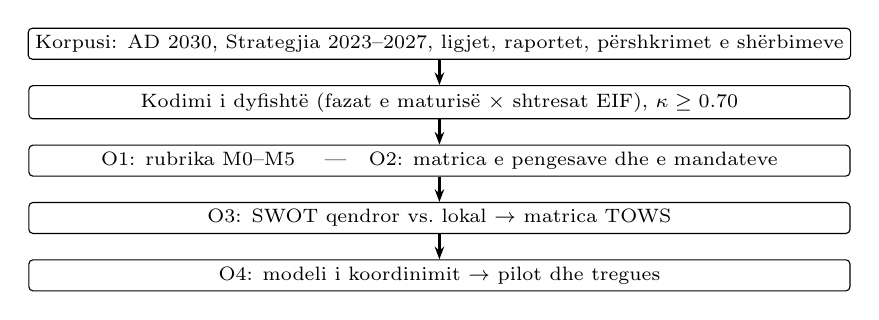
\begin{tikzpicture}[
  node distance=3.2mm,
  box/.style={draw, rounded corners=1.5pt, align=center, font=\scriptsize,
              minimum width=0.86\columnwidth, inner sep=2.5pt},
  arr/.style={-{Stealth[length=1.6mm]}, thick}]
\node[box] (a) {Korpusi: AD~2030, Strategjia 2023--2027, ligjet,
raportet, përshkrimet e shërbimeve};
\node[box, below=of a] (b) {Kodimi i dyfishtë (fazat e maturisë $\times$
shtresat EIF), $\kappa \geq 0.70$};
\node[box, below=of b] (c) {O1: rubrika M0--M5 \quad|\quad O2: matrica e
pengesave dhe e mandateve};
\node[box, below=of c] (d) {O3: SWOT qendror vs.\ lokal $\rightarrow$ matrica
TOWS};
\node[box, below=of d] (e) {O4: modeli i koordinimit $\rightarrow$ pilot
dhe tregues};
\draw[arr] (a) -- (b);
\draw[arr] (b) -- (c);
\draw[arr] (c) -- (d);
\draw[arr] (d) -- (e);
\end{tikzpicture}
\caption{Rrjedha metodologjike dhe lidhja me objektivat O1--O4.}
\label{fig:metodologjia}
\end{figure}
% ---------------------------------------------------------------------
% 8. TEKNOLOGJITË DHE VEGLAT
% ---------------------------------------------------------------------
\section{Teknologjitë dhe veglat e punës}
\label{sec:veglat}
Dallojmë dy grupe: teknologjitë që janë \textit{objekt} i analizës dhe
veglat që përdoren \textit{për} analizë (Tabela~\ref{tab:veglat}). Te grupi i
parë, e-Kosova shqyrtohet përmes përshkrimeve publike të shërbimeve për të
identifikuar çfarë bën qytetari në portal, ndërsa dokumentacioni
institucional për \textit{Government Gateway} dhe regjistrat përkatës
përdoret për të verifikuar nëse dhe si shkëmbehen të dhënat. Analiza kryhet
vetëm me materiale publike, pa përdorur llogari ose të dhëna personale të
qytetarëve. Te grupi i dytë, rrjedhat e proceseve modelohen në notacionin
BPMN~2.0 me korsi të veçanta për qytetarin, komunën dhe institucionin
qendror, në mënyrë që të bëhet i dukshëm hapi ku përgjegjësia kalon nga
njëra palë te tjetra.

\begin{table}[!t]
\caption{Teknologjitë e analizuara dhe veglat e hulumtimit}
\label{tab:veglat}
\centering
\footnotesize
\renewcommand{\arraystretch}{1.15}
\begin{tabular}{L{0.32\columnwidth} L{0.58\columnwidth}}
\toprule
\textbf{Teknologjia / vegla} & \textbf{Roli në punim} \\
\midrule
\multicolumn{2}{l}{\textit{Objekt i analizës}} \\
e-Kosova & Pika e hyrjes së qytetarit; nivelet M1--M3 \\
\textit{Government Gateway} & Shkëmbimi ndërmjet regjistrave; nivelet M4--M5 \\
eID dhe shërbimet e besuara & Shtresa ligjore-teknike e identifikimit
(Ligji 08/L-022) \\
Rrjeti qeveritar, qendra e të dhënave & Mundësuesit e përbashkët dhe
varësia nga partnerët \\
\midrule
\multicolumn{2}{l}{\textit{Vegla të hulumtimit}} \\
Zotero & Menaxhimi i referencave, DOI-ve dhe shënimeve të leximit \\
Microsoft Excel & Matrica e kodimit: një rresht për çdo hap procesi,
i lidhur me dokumentin, faqen, institucionin dhe shtresën EIF \\
Python (pandas, scikit-learn) & Llogaritja e $\kappa$-së së Cohen-it dhe
gjenerimi i riprodhueshëm i tabelave \\
diagrams.net (BPMN~2.0) & Modelimi i proceseve me korsi
qytetar--komunë--qendër \\
Crossref API & Verifikimi i metadatave dhe DOI-ve të referencave \\
\LaTeX{} / Overleaf & Shkrimi bashkëpunues dhe versionimi i punimit \\
\bottomrule
\end{tabular}
\end{table}
% ---------------------------------------------------------------------
% 9. PËRSHKRIMI I PROBLEMIT DHE REZULTATET E PRITURA
% ---------------------------------------------------------------------
\section{Përshkrimi i problemit dhe rezultatet e pritura}
\label{sec:problemi}
\subsection{Përshkrimi i problemit}
Problemi nis aty ku kompetenca për të ofruar një shërbim dhe kompetenca për
të ndryshuar të dhënat e tij u takojnë institucioneve të ndryshme. Ta marrim
si shembull një qytetar që shkarkon nga e-Kosova një ekstrakt të gjendjes
civile dhe vëren një pasaktësi. Dokumenti është lëshuar elektronikisht, por
qytetarit ende i duhet të dijë (i) ku ta paraqesë kërkesën për korrigjim,
(ii) kush ka kompetencë ta përditësojë regjistrin -- meqë regjistrimi civil
është kompetencë e deleguar te komunat \cite{ligji03L040} -- dhe (iii) si do
ta marrë dokumentin e saktë. Në terma të rubrikës, procesi duket M3 nga ana e
qytetarit, por mund të jetë M2 ose më poshtë nga ana e administratës. Ky
\textit{hendek ndërmjet maturisë së dukshme dhe asaj të dëshmuar} është
problemi qendror i punimit dhe vlen edhe për shërbime të tjera.

Në nivel qendror shqyrtohet kush përcakton rregullat e përbashkëta për
shkëmbimin e të dhënave dhe kush vendos kur dy institucione i interpretojnë
ato ndryshe. Në nivel komunal shqyrtohet nëse zyrtari ka udhëzim të
mjaftueshëm për ta përcjellë rastin dhe për ta njoftuar qytetarin, duke i
lexuar faktorët e zbatimit brenda administratës së bashku me ata të pranimit
nga qytetarët \cite{gilgarcia2020}. Kur një
procedurë nuk është e përshkruar në dokumentet publike, raportohet kufiri i
dokumentacionit dhe përcaktohet çfarë dëshmie do të duhej për ta verifikuar
praktikën.

\subsection{Vlerësimi i modelit aktual: gjendja dhe rekomandime}
Tabela~\ref{tab:vleresimi} paraqet vlerësimin paraprak të modelit, të
nxjerrë nga dokumentet strategjike para kodimit të plotë të proceseve. Ai
sugjeron një profil ``të shtrembër'': prania informative dhe disa
transaksione janë konsoliduar, por integrimi vertikal dhe horizontal mbetet
në fazë fillestare, ndërsa mundësuesit institucionalë dhe matja janë hallkat
më të dobëta. Ky profil përputhet me gjetjen se maturia është konfiguracionale
dhe jo lineare \cite{iannacci2025}: investimet në kanalin e qytetarit nuk
përkthehen automatikisht në integrim të brendshëm.

\begin{table*}[!t]
\caption{Vlerësimi paraprak i modelit aktual të e-Qeverisjes në Kosovë
(i bazuar në dokumente; do të rifreskohet pas kodimit të plotë)}
\label{tab:vleresimi}
\centering
\footnotesize
\renewcommand{\arraystretch}{1.2}
\begin{tabularx}{\textwidth}{L{0.15\textwidth} Y L{0.13\textwidth} Y}
\toprule
\textbf{Dimensioni} & \textbf{Dëshmia kryesore} & \textbf{Gjendja paraprake}
& \textbf{Rekomandimi} \\
\midrule
Prania informative & e-Kosova si dritare e vetme për të gjitha nivelet
\cite{strategjia2023} & M1 e konsoliduar & R1: katalog i unifikuar i
shërbimeve me pronar institucional dhe bazë ligjore për çdo shërbim \\
Transaksionet & $\approx$10\% e mbi 700 shërbimeve online; 5.3\% dorëzim
formularësh \cite{strategjia2023,agjenda2030} & M3 e pjesshme dhe e
fragmentuar & R2: prioritizim i ridizajnit sipas vëllimit të kërkesave,
jo sipas institucionit \\
Integrimi vertikal & Kompetenca komunale vetanake e të deleguara
\cite{ligji03L040}; niveli lokal pa përfaqësim të dedikuar në strukturat e
zbatimit \cite{strategjia2023} & M4 e kufizuar / e padokumentuar & R3:
përfaqësim i komunave në komitetin teknik dhe udhëzime procedurale
qendër--komunë \\
Integrimi horizontal & \textit{Government Gateway} që nga 2017; synim 30\%
$\rightarrow$ 70\% e sistemeve të lidhura; metadata të paharmonizuara, pa
arkitekturë të ndërmarrjes \cite{strategjia2023} & M5 në fazë fillestare &
R4: katalog semantik i të dhënave bazë dhe parimi \textit{once-only} sipas
EIF \cite{eif2017} \\
Mundësuesit institucionalë & GTEI 0.456 (C); $\approx$450 specialistë TI
(0.5\%); role të paqarta e të mbivendosura \cite{strategjia2023} & I dobët &
R5: matricë RACI e mandateve dhe plan për kapacitetet e brendshme të TI-së \\
Matja dhe monitorimi & Jashtë EGDI e DESI; shumë vlera bazë ``N/A''
\cite{undesa2024,agjenda2030,strategjia2023} & Deficit strukturor & R6:
Pasaportë e Treguesve me përkufizime operacionale dhe matje në nivel procesi
\\
\bottomrule
\end{tabularx}
\end{table*}

Rekomandimet R1--R6 janë të renditura sipas varësisë logjike: R5 dhe R6 janë
parakushte, sepse pa mandate të qarta dhe pa matje, as ridizajni i shërbimeve
(R2) dhe as integrimi (R3--R4) nuk mund të vlerësohen. Secili rekomandim
lidhet me një dimension të vlerës publike \cite{twizeyimana2019} --
përmirësim i shërbimit (R1--R2), efikasitet administrativ (R3--R5) dhe
llogaridhënie (R6).

\subsection{Analiza SWOT e nivelit qendror dhe lokal}
Tabela~\ref{tab:swot} paraqet faktorët SWOT paraprakë për të dy nivelet.
Asimetria është e qartë: niveli qendror zotëron mundësuesit strategjikë dhe
ligjorë, por vuan nga fragmentimi horizontal; niveli lokal është më afër
qytetarit dhe mban kompetenca kyçe (p.sh., regjistrimin civil), por varet nga
sistemet qendrore dhe nuk ka zë të institucionalizuar në vendimmarrje. Kjo
përputhet me dëshmitë ndërkombëtare për kufizimet e zbatimit në nivel lokal
\cite{kuhlmann2023,pekkola2022}.

\begin{table*}[!t]
\caption{Analiza SWOT paraprake e e-Qeverisjes në nivel qendror dhe lokal}
\label{tab:swot}
\centering
\footnotesize
\renewcommand{\arraystretch}{1.2}
\begin{tabularx}{\textwidth}{L{0.10\textwidth} Y Y}
\toprule
& \textbf{Niveli qendror} & \textbf{Niveli lokal (38 komuna)} \\
\midrule
\textbf{S} -- Pikat e forta &
Vazhdimësi strategjike 2009--2030; kornizë ligjore e përafruar me eIDAS dhe
GDPR; \textit{Government Gateway} funksional që nga 2017; Komision për
Transformim Digjital i kryesuar nga Kryeministri; kalim nga grupi C në B në
GTMI \cite{strategjia2023,agjenda2030} &
Afërsi me qytetarin dhe njohje e rasteve konkrete; kompetenca vetanake dhe
të deleguara (p.sh., regjistrimi civil) \cite{ligji03L040}; qasje përmes
e-Kosova si dritare e përbashkët \cite{strategjia2023} \\
\midrule
\textbf{W} -- Dobësitë &
Portale të fragmentuara; metadata të paharmonizuara; pa inventar të
sistemeve TI dhe pa arkitekturë të ndërmarrjes; role të paqarta e të
mbivendosura; GTEI 0.456; $\approx$450 specialistë TI (0.5\%)
\cite{strategjia2023} &
Kapacitete digjitale të pabarabarta; mungesë përfaqësimi të dedikuar në
strukturat e zbatimit \cite{strategjia2023}; ndërprerje teknike të
raportuara nga qytetarët dhe drejtuesit komunalë \cite{mustafa2022} \\
\midrule
\textbf{O} -- Mundësitë &
Procesi i anëtarësimit në BE dhe përafrimi me EIF \cite{ec2024,eif2017};
mbështetje teknike nga Estonia \cite{strategjia2023,kalvet2012}; buxhet
indikativ 152 mln euro \cite{agjenda2030} &
Standarde dhe shërbime të përbashkëta qendrore që ulin koston e
digjitalizimit lokal; lidhje pozitive kënaqësi--efikasitet te përdoruesit
e e-Kosova \cite{sherifi2026}; modele bashkëpunimi ndërkomunal
\cite{wouters2023} \\
\midrule
\textbf{T} -- Kërcënimet &
Varësi nga partnerët e jashtëm për mundësuesit kryesorë; 35\% e buxhetit nga
donatorët \cite{strategjia2023,agjenda2030}; kërcënime kibernetike dhe
akterë të shpërndarë të sigurisë \cite{kipred2022} &
Përdorim i ulët (72\% pa ndërveprim online me administratën)
\cite{oecd2024}; besim dhe aftësi digjitale të kufizuara \cite{krasniqi2026};
rrezik i ``digjitalizimit me dy shpejtësi'' ndërmjet komunave \\
\bottomrule
\end{tabularx}
\end{table*}

Matrica TOWS (Tabela~\ref{tab:tows}) i kthen këta faktorë në opsione
strategjike. Strategjitë WO dhe WT janë më të rëndësishmet për rastin
kosovar, sepse dobësitë institucionale, e jo mungesa e mundësive, janë
kufizimi dominues.

\begin{table}[!t]
\caption{Matrica TOWS paraprake (opsione strategjike)}
\label{tab:tows}
\centering
\footnotesize
\renewcommand{\arraystretch}{1.15}
\begin{tabular}{L{0.10\columnwidth} L{0.80\columnwidth}}
\toprule
\textbf{Çifti} & \textbf{Opsioni strategjik} \\
\midrule
SO & Përdorimi i \textit{Government Gateway} dhe i përafrimit me EIF për
të lidhur me prioritet regjistrat që përdoren nga komunat \\
WO & Shfrytëzimi i procesit të integrimit në BE për katalog semantik,
arkitekturë të ndërmarrjes dhe matricë RACI të mandateve \\
ST & Ndërtimi i kapaciteteve të brendshme për mundësuesit kryesorë, për ta
ulur varësinë nga partnerët dhe donatorët \\
WT & Përfaqësimi i komunave në komitetin teknik dhe një pikë kontakti
qendër--komunë për çdo proces të përbashkët \\
\bottomrule
\end{tabular}
\end{table}

\subsection{Rezultatet e pritura}
Rezultatet e pritura lidhen një-për-një me objektivat
(Tabela~\ref{tab:objmet}). \textit{Për O1}, pritet një pasqyrë e maturisë
në nivel procesi, ku lexuesi sheh sa larg ndiqet kërkesa në dokumente dhe në
cilin hap hyn një institucion tjetër. \textit{Për O2}, pritet një tabelë e
mandateve që tregon kush i mban të dhënat, kush vendos për to dhe kujt i
drejtohet qytetari për sqarim, e kryqëzuar me shtresat e EIF-it.
\textit{Për O3}, presim të dallojmë faktorët me peshë të ndryshme në të dy
nivelet; p.sh., një standard i përbashkët e lehtëson punën e komunës vetëm
nëse zyra ka personel të trajnuar, dhe ky kombinim hyn në TOWS vetëm nëse të
dy faktorët dokumentohen.

\textit{Për O4}, propozohet një mekanizëm koordinimi i testueshëm fillimisht
në një proces pilot (p.sh., korrigjimi i të dhënave të gjendjes civile):
komuna dhe institucioni qendror caktojnë nga një pikë kontakti, një afat
përgjigjeje dhe një kanal për njoftimin e qytetarit kur rasti mbyllet.
Performanca matet me dy tregues: (i) koha mediane nga përcjellja e rastit
deri te përgjigjja dhe (ii) përqindja e rasteve të mbyllura pa vizitë
shtesë në sportel, e llogaritur mbi të gjitha rastet e mbyllura në të
njëjtën periudhë, ndërsa rastet e hapura raportohen veçmas. Vlerat bazë dhe
synimet përcaktohen vetëm pasi të sigurohen të dhëna të krahasueshme, në
përputhje me rregullin e krahasueshmërisë të Seksionit~\ref{sec:metodat}.

\begin{table}[!t]
\caption{Lidhja objektiv--metodë--rezultat i pritur}
\label{tab:objmet}
\centering
\footnotesize
\renewcommand{\arraystretch}{1.15}
\begin{tabular}{L{0.08\columnwidth} L{0.36\columnwidth} L{0.44\columnwidth}}
\toprule
\textbf{Obj.} & \textbf{Metoda} & \textbf{Rezultati i pritur} \\
\midrule
O1 & Rubrika M0--M5, kodim i dyfishtë & Pasqyra e maturisë për çdo proces,
qendror dhe lokal \\
O2 & Kodimi i pengesave sipas EIF & Matrica e mandateve dhe e pengesave
(ligjore, organizative, semantike, teknike) \\
O3 & SWOT me gjurmim burimesh, TOWS & SWOT qendror vs.\ lokal dhe opsione
strategjike me pronar \\
O4 & Dizajn mbi mekanizma të dëshmuar, pilot & Model koordinimi me role,
afate dhe dy tregues performance \\
\bottomrule
\end{tabular}
\end{table}
% ---------------------------------------------------------------------
% 10. REFERENCAT (renditur sipas citimit të parë, stili IEEE)
% DOI-të e punimeve shkencore janë verifikuar përmes Crossref (11/2026).
% ---------------------------------------------------------------------
\begin{thebibliography}{00}
\bibitem{mergel2019} I. Mergel, N. Edelmann, and N. Haug, ``Defining digital transformation: Results from expert interviews,'' \emph{Government Information Quarterly}, vol. 36, no. 4, art. 101385, 2019, doi: 10.1016/j.giq.2019.06.002.
\bibitem{janowski2015} T. Janowski, ``Digital government evolution: From transformation to contextualization,'' \emph{Government Information Quarterly}, vol. 32, no. 3, pp. 221--236, 2015, doi: 10.1016/j.giq.2015.07.001.
\bibitem{glyptis2020} L. Glyptis, M. Christofi, D. Vrontis, M. Del Giudice, S. Dimitriou, and P. Michael, ``E-Government implementation challenges in small countries: The project manager's perspective,'' \emph{Technological Forecasting and Social Change}, vol. 152, art. 119880, 2020, doi: 10.1016/j.techfore.2019.119880.
\bibitem{strategjia2023} Qeveria e Republikës së Kosovës, \emph{Strategjia e Kosovës për Qeverisje Elektronike 2023--2027}, versioni final, Prishtinë, Kosovë, 2023.
\bibitem{agjenda2030} Ministria e Ekonomisë, \emph{Agjenda Digjitale e Kosovës 2030}, Prishtinë, Kosovë, 2023.
\bibitem{ec2024} European Commission, ``Kosovo 2024 Report,'' Commission Staff Working Document, Brussels, Belgium, 2024.
\bibitem{eif2017} European Commission, ``New European Interoperability Framework: Promoting seamless services and data flows for European public administrations,'' COM(2017) 134 final, Luxembourg: Publications Office of the European Union, 2017.
\bibitem{oecd2024} OECD, \emph{Western Balkans Competitiveness Outlook 2024: Kosovo}. Paris, France: OECD Publishing, 2024.
\bibitem{ligji03L040} Kuvendi i Republikës së Kosovës, ``Ligji Nr. 03/L-040 për Vetëqeverisjen Lokale,'' \emph{Gazeta Zyrtare e Republikës së Kosovës}, 2008.
\bibitem{kipred2022} L. Peci and V. Ukshini, \emph{Qeverisja e mirë në sigurinë kibernetike në Kosovë: Forcimi i themeleve dhe i institucioneve të reja}. Prishtinë, Kosovë: KIPRED/DCAF, Sep. 2022.
\bibitem{undesa2024} United Nations Department of Economic and Social Affairs, \emph{United Nations E-Government Survey 2024: Accelerating Digital Transformation for Sustainable Development}. New York, NY, USA: United Nations, 2024.
\bibitem{dermaku2024} K. Dërmaku and A. Emini, ``Digitisation of administration and legal basis in Kosovo,'' \emph{Access to Justice in Eastern Europe}, vol. 7, no. 1, pp. 245--263, 2024, doi: 10.33327/AJEE-18-7.1-a000107.
\bibitem{krasniqi2026} M. Krasniqi, Z. Elezi, and D. Vuniqi, ``The digitalization of public administration in Kosovo: Challenges, opportunities and the impact on the quality of public services,'' \emph{Prizren Social Science Journal}, vol. 10, no. 2, pp. 165--177, 2026, doi: 10.32936/pssj.v10i2.880.
\bibitem{pardo2012} T. A. Pardo, T. Nam, and G. B. Burke, ``E-government interoperability: Interaction of policy, management, and technology dimensions,'' \emph{Social Science Computer Review}, vol. 30, no. 1, pp. 7--23, 2012, doi: 10.1177/0894439310392184.
\bibitem{layne2001} K. Layne and J. Lee, ``Developing fully functional E-government: A four stage model,'' \emph{Government Information Quarterly}, vol. 18, no. 2, pp. 122--136, 2001, doi: 10.1016/S0740-624X(01)00066-1.
\bibitem{iannacci2025} F. Iannacci, S. Karanasios, G. Viscusi, R. McManus, C. Rupietta, and C. W. Tan, ``Unboxing maturity models: A set-theoretic perspective on e-Government configurations over time,'' \emph{The Journal of Strategic Information Systems}, vol. 34, no. 1, art. 101874, 2025, doi: 10.1016/j.jsis.2024.101874.
\bibitem{kalvet2012} T. Kalvet, ``Innovation: A factor explaining e-government success in Estonia,'' \emph{Electronic Government, an International Journal}, vol. 9, no. 2, pp. 142--157, 2012, doi: 10.1504/EG.2012.046266.
\bibitem{yin2018} R. K. Yin, \emph{Case Study Research and Applications: Design and Methods}, 6th ed. Thousand Oaks, CA, USA: SAGE, 2018.
\bibitem{bowen2009} G. A. Bowen, ``Document analysis as a qualitative research method,'' \emph{Qualitative Research Journal}, vol. 9, no. 2, pp. 27--40, 2009, doi: 10.3316/QRJ0902027.
\bibitem{mchugh2012} M. L. McHugh, ``Interrater reliability: The kappa statistic,'' \emph{Biochemia Medica}, vol. 22, no. 3, pp. 276--282, 2012, doi: 10.11613/BM.2012.031.
\bibitem{scholta2019} H. Scholta, W. Mertens, M. Kowalkiewicz, and J. Becker, ``From one-stop shop to no-stop shop: An e-government stage model,'' \emph{Government Information Quarterly}, vol. 36, no. 1, pp. 11--26, 2019, doi: 10.1016/j.giq.2018.11.010.
\bibitem{campmas2022} A. Campmas, N. Iacob, and F. Simonelli, ``How can interoperability stimulate the use of digital public services? An analysis of national interoperability frameworks and e-Government in the European Union,'' \emph{Data \& Policy}, vol. 4, art. e19, 2022, doi: 10.1017/dap.2022.11.
\bibitem{weihrich1982} H. Weihrich, ``The TOWS matrix -- A tool for situational analysis,'' \emph{Long Range Planning}, vol. 15, no. 2, pp. 54--66, 1982, doi: 10.1016/0024-6301(82)90120-0.
\bibitem{wouters2023} S. Wouters, M. Janssen, V. Lember, and J. Crompvoets, ``Strategies to advance the dream of integrated digital public service delivery in inter-organizational collaboration networks,'' \emph{Government Information Quarterly}, vol. 40, no. 1, art. 101779, 2023, doi: 10.1016/j.giq.2022.101779.
\bibitem{fusi2021} F. Fusi, ``When local governments request access to data: Power and coordination mechanisms across stakeholders,'' \emph{Public Administration Review}, vol. 81, no. 1, pp. 23--37, 2021, doi: 10.1111/puar.13307.
\bibitem{gilgarcia2020} J. R. Gil-Garcia and M. Á. Flores-Zúñiga, ``Towards a comprehensive understanding of digital government success: Integrating implementation and adoption factors,'' \emph{Government Information Quarterly}, vol. 37, no. 4, art. 101518, 2020, doi: 10.1016/j.giq.2020.101518.
\bibitem{twizeyimana2019} J. D. Twizeyimana and A. Andersson, ``The public value of E-Government -- A literature review,'' \emph{Government Information Quarterly}, vol. 36, no. 2, pp. 167--178, 2019, doi: 10.1016/j.giq.2019.01.001.
\bibitem{kuhlmann2023} S. Kuhlmann and M. Heuberger, ``Digital transformation going local: Implementation, impacts and constraints from a German perspective,'' \emph{Public Money \& Management}, vol. 43, no. 2, pp. 147--155, 2023, doi: 10.1080/09540962.2021.1939584.
\bibitem{pekkola2022} S. Pekkola, M. Ylinen, and N. Mavengere, ``Consortium of municipalities co-tailoring a governmental e-service platform: What could go wrong?'' \emph{Digital Government: Research and Practice}, vol. 3, no. 1, art. 6, 2022, doi: 10.1145/3511889.
\bibitem{mustafa2022} N. Mustafa, A. Bajrami, and X. Islami, ``Electronic services management in local governance -- Evidence from a transitional economy,'' \emph{International Journal of Sustainable Development and Planning}, vol. 17, no. 2, pp. 615--621, 2022, doi: 10.18280/ijsdp.170226.
\bibitem{sherifi2026} Z. Sherifi and K. Krasniqi, ``The effect of the E-Kosova platform on enhancing public services for citizens in Kosovo,'' in \emph{AI and Digital Transformation: Opportunities, Challenges, and Emerging Threats in Technology, Business, and Security}, CCIS, vol. 2670. Cham, Switzerland: Springer, 2026, pp. 253--266, doi: 10.1007/978-3-032-07370-9\_18.
\end{thebibliography}
\end{document}
